\documentclass[11pt]{article}
\usepackage[margin=0.78in]{geometry}
\usepackage[T1]{fontenc}
\usepackage[utf8]{inputenc}
\usepackage{lmodern,microtype}
\usepackage{amsmath,amssymb,mathtools}
\usepackage{booktabs,array,longtable,enumitem}
\usepackage{xcolor,hyperref}
\usepackage{tikz}
\usepackage[most]{tcolorbox}
\usetikzlibrary{arrows.meta,positioning,calc}
\hypersetup{colorlinks=true,linkcolor=blue!50!black,urlcolor=blue!50!black,pdftitle={PMSM, FOC, and Grid Inverter Integration Guide}}
\setlength{\parskip}{4pt}
\setlength{\parindent}{0pt}
\setlist[itemize]{topsep=2pt,itemsep=2pt,leftmargin=*}
\renewcommand{\arraystretch}{1.18}
\definecolor{MSBlue}{RGB}{19,72,112}
\definecolor{MSGreen}{RGB}{25,112,85}
\definecolor{SoftBlue}{RGB}{237,246,253}
\definecolor{SoftGreen}{RGB}{238,249,242}
\definecolor{SoftYellow}{RGB}{255,249,231}
\definecolor{SoftRed}{RGB}{255,241,240}
\newtcolorbox{keybox}[1]{enhanced,breakable,colback=SoftBlue,colframe=MSBlue,title=\textbf{#1},arc=1.5mm,boxrule=0.65pt}
\newtcolorbox{examplebox}[1]{enhanced,breakable,colback=SoftYellow,colframe=orange!65!black,title=\textbf{Worked example: #1},arc=1.5mm,boxrule=0.65pt}
\newtcolorbox{warningbox}[1]{enhanced,breakable,colback=SoftRed,colframe=red!55!black,title=\textbf{Integration caution: #1},arc=1.5mm,boxrule=0.65pt}
\newtcolorbox{checklistbox}[1]{enhanced,breakable,colback=SoftGreen,colframe=MSGreen,title=\textbf{#1},arc=1.5mm,boxrule=0.65pt}
\newcommand{\jop}{\mathrm{j}}
\newcommand{\V}{\mathrm{V}}
\newcommand{\A}{\mathrm{A}}
\newcommand{\Hz}{\mathrm{Hz}}
\newcommand{\kW}{\mathrm{kW}}
\newcommand{\kVA}{\mathrm{kVA}}
\newcommand{\ohm}{\Omega}
\title{\textbf{PMSM, Field-Oriented Control, and Grid Inverter Integration}\\\large A technical guide for Linear Generator and inverter-systems integration work}
\author{Study Guide}
\date{\today}
\begin{document}
\maketitle
\begin{abstract}
PMSM and field-oriented-control experience is highly transferable to a grid-interactive power-conversion role, but the controlled plant and operating objectives change. This guide develops the common inverter foundation, then translates motor-drive concepts into grid-following and grid-forming inverter control, protection, validation, and field diagnostics. Product-specific Linear Generator internals are proprietary; Mainspring public material describes pressure-driven oscillators, coils, and power electronics at a system level.
\end{abstract}
\tableofcontents
\newpage

\section{Where PMSM Knowledge Transfers}
\subsection{The correct comparison}
A PMSM converts electrical energy into rotary mechanical energy. A linear generator converts externally supplied reciprocating mechanical motion into electrical energy. Both may use permanent magnets, copper windings, position-dependent flux linkage, and PWM power electronics, but they are not the same machine.

\begin{center}
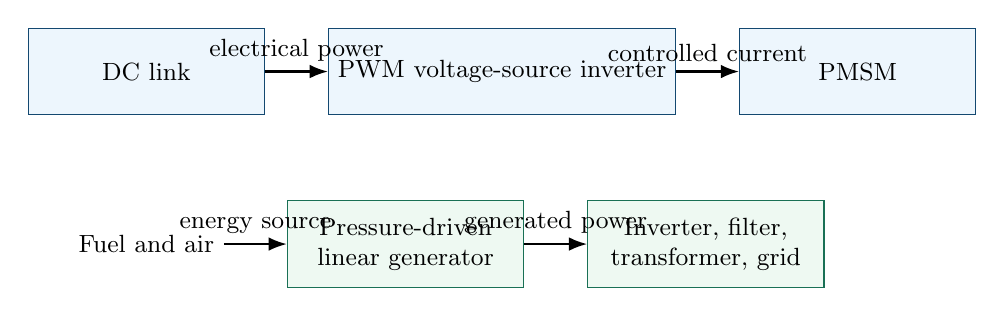
\begin{tikzpicture}[>=Latex,node distance=8mm,every node/.style={font=\small}]
\tikzset{block/.style={draw=MSBlue,fill=SoftBlue,minimum width=30mm,minimum height=11mm,align=center},gblock/.style={draw=MSGreen,fill=SoftGreen,minimum width=30mm,minimum height=11mm,align=center}}
\node[block] (dc) {DC link};
\node[block,right=of dc] (vsi) {PWM voltage-source inverter};
\node[block,right=of vsi] (motor) {PMSM};
\node[below=14mm of dc] (fuel) {Fuel and air};
\node[gblock,right=of fuel] (lg) {Pressure-driven\\linear generator};
\node[gblock,right=of lg] (gridinv) {Inverter, filter,\\transformer, grid};
\draw[->,thick] (dc)--node[above]{electrical power}(vsi);
\draw[->,thick] (vsi)--node[above]{controlled current}(motor);
\draw[->,thick] (fuel)--node[above]{energy source}(lg);
\draw[->,thick] (lg)--node[above]{generated power}(gridinv);
\end{tikzpicture}
\end{center}

The transferable control stack is: calibrated sensing, synchronous reference frame, current regulation, PWM, timing discipline, saturation handling, fault protection, and test evidence. The major translation is from \emph{torque and speed} to \emph{real/reactive power, voltage, frequency, and grid-code behavior}.

\begin{longtable}{p{0.27\linewidth}p{0.29\linewidth}p{0.32\linewidth}}
\toprule
PMSM drive concept & Grid-following inverter analogue & Engineering implication \\
\midrule
Rotor electrical angle & Grid angle estimated by PLL & Bad angle estimation corrupts $dq$ currents. \\
Torque command & Active-power current command & Current limit bounds delivered power. \\
Speed outer loop & DC-bus voltage or active-power outer loop & Slower than the current loop. \\
Machine inductance & Filter plus grid impedance & Varies with cable, transformer, and grid. \\
Mechanical load step & Grid sag, frequency event, or site-load step & Requires ride-through and stable limiting. \\
Back-EMF & Grid voltage & The inverter must synthesize a voltage relative to it. \\
\bottomrule
\end{longtable}

\section{Three-Phase Inverter Hardware}
\subsection{Voltage-source inverter and PWM}
A two-level, three-phase voltage-source inverter (VSI) uses six controlled switches and antiparallel current paths to connect each phase to the positive or negative DC rail. Pulse-width modulation makes the average phase voltage follow a commanded sinusoidal reference. For a sinusoidal PWM approximation in the linear modulation region,
\[
V_{ph,1,peak}\approx \frac{m_aV_{dc}}{2},\qquad 0\leq m_a\leq1,
\]
where $m_a$ is modulation index. Space-vector PWM uses the same physical switching states but allocates zero-vector time more effectively and commonly provides better DC-bus utilization.

Dead time protects against shoot-through, yet distorts current near zero crossing. It must be characterized or compensated using current polarity, switch timing, and measured waveform evidence.

\subsection{DC link, switching losses, and thermal path}
The DC link buffers the mismatch between source power and AC-side power:
\[
C_{dc}\frac{dV_{dc}}{dt}=\frac{P_{src}-P_{ac}-P_{loss}}{V_{dc}}.
\]
Its capacitor must tolerate voltage, ripple current, temperature, expected life, and transients. Precharge limits inrush into this capacitance before a main contactor closes.

An approximate semiconductor loss model is
\[
P_{loss}=P_{cond}+P_{sw},\qquad P_{sw}\approx f_s(E_{on}+E_{off}),
\]
where switching energies depend on current, voltage, device temperature, and gate drive. Junction temperature follows the complete thermal chain:
\[
T_j=T_a+P_{loss}(R_{\theta jc}+R_{\theta cs}+R_{\theta sa}).
\]
IGBTs often favor high-power moderate-switching-frequency designs; SiC MOSFETs can reduce switching loss and enable higher frequency, but layout, gate drive, insulation stress, and EMI must be designed accordingly.

\begin{examplebox}{DC-bus current}
For a $250\,\kW$ converter supplied from a $1000\,\V$ DC bus at $97\%$ converter efficiency,
\[
I_{dc}\approx\frac{250000}{0.97(1000)}=258\,\A.
\]
This is only the average value. Capacitor ripple-current capability, transient current, fault interruption, and busbar inductance remain separate requirements.
\end{examplebox}

\subsection{Output filters and sensing}
An L filter limits switching-current ripple. An LCL filter reduces high-frequency harmonic injection more strongly, but its resonance must be damped and kept away from control bandwidth and uncertain grid resonances. A first estimate is
\[
f_r=\frac{1}{2\pi}\sqrt{\frac{L_1+L_2}{L_1L_2C_f}}.
\]
Phase-current sensors require polarity checks, offset removal, gain calibration, adequate bandwidth, saturation margin, and a defined failure response. A sign error can turn negative feedback into positive feedback; treat first energization as a controlled, low-power verification rather than a production run.

\section{PMSM Model and Field-Oriented Control}
\subsection{Reference-frame transformations}
Balanced three-phase currents can be represented as a stationary two-axis vector through the Clarke transform:
\[
\begin{bmatrix}i_\alpha\\i_\beta\end{bmatrix}=
\frac{2}{3}
\begin{bmatrix}1&-1/2&-1/2\\0&\sqrt3/2&-\sqrt3/2\end{bmatrix}
\begin{bmatrix}i_a\\i_b\\i_c\end{bmatrix}.
\]
The Park transform rotates that vector by electrical angle $\theta_e$:
\[
\begin{bmatrix}i_d\\i_q\end{bmatrix}=
\begin{bmatrix}\cos\theta_e&\sin\theta_e\\-\sin\theta_e&\cos\theta_e\end{bmatrix}
\begin{bmatrix}i_\alpha\\i_\beta\end{bmatrix}.
\]
For a correctly aligned frame, sinusoidal steady-state currents become nearly DC quantities. PI regulators can then track current commands without trying to regulate a sinusoid directly.

\subsection{PMSM $dq$ equations and torque}
For a PMSM with electrical speed $\omega_e$,
\[
v_d=R_si_d+L_d\frac{di_d}{dt}-\omega_eL_qi_q,
\]
\[
v_q=R_si_q+L_q\frac{di_q}{dt}+\omega_e(L_di_d+\lambda_m).
\]
The cross-coupling terms motivate feedforward decoupling. Electromagnetic torque is
\[
T_e=\frac{3}{2}p\left[\lambda_m i_q+(L_d-L_q)i_di_q\right],
\]
where $p$ is pole-pair count and $\lambda_m$ is PM flux linkage. Surface-PM machines commonly use $i_d\approx0$ below base speed; salient interior-PM machines can exploit negative $i_d$ for maximum torque per ampere (MTPA).

Above base speed, back-EMF consumes voltage headroom. Field weakening applies negative $i_d$ so the voltage magnitude remains feasible:
\[
v_d^2+v_q^2\leq V_{max}^2.
\]
Current is separately constrained:
\[
i_d^2+i_q^2\leq I_{max}^2.
\]
These two circles are a useful mental model for every limited inverter, including a grid converter during a voltage event.

\subsection{Current-loop implementation}
The usual hierarchy is a fast $d/q$ current loop inside a slower torque or speed loop. A PI law may be written as
\[
v_d^*=K_{pd}(i_d^*-i_d)+K_{id}\int(i_d^*-i_d)dt+v_{d,ff},
\]
with an equivalent $q$ axis equation. Actual behavior depends on ADC sampling instant, computation delay, PWM update, sensor filtering, voltage saturation, and anti-windup. A clean simulation without these effects is not enough to establish hardware stability.

\section{From FOC to Grid-Following Inverters}
\subsection{PLL and $dq$ power control}
A grid-following inverter uses a phase-locked loop (PLL) to estimate grid angle. With the $d$ axis aligned to grid voltage, $v_q\approx0$, and three-phase power becomes
\[
P=\frac{3}{2}v_di_d,\qquad Q=-\frac{3}{2}v_di_q,
\]
under this stated sign convention. Different firmware may define axes or reactive-power signs differently; verify conventions in its interface control document and test data.

\begin{center}
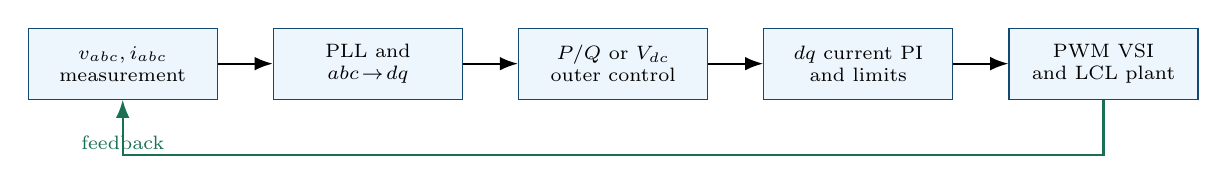
\begin{tikzpicture}[>=Latex,node distance=7mm,every node/.style={font=\scriptsize}]
\tikzset{block/.style={draw=MSBlue,fill=SoftBlue,minimum width=24mm,minimum height=9mm,align=center}}
\node[block] (meas) {$v_{abc},i_{abc}$\\measurement};
\node[block,right=of meas] (pll) {PLL and\\$abc\!\to\!dq$};
\node[block,right=of pll] (outer) {$P/Q$ or $V_{dc}$\\outer control};
\node[block,right=of outer] (current) {$dq$ current PI\\and limits};
\node[block,right=of current] (pwm) {PWM VSI\\and LCL plant};
\draw[->,thick](meas)--(pll); \draw[->,thick](pll)--(outer); \draw[->,thick](outer)--(current); \draw[->,thick](current)--(pwm);
\draw[->,thick,MSGreen](pwm.south) |- ++(0,-7mm) -| node[pos=.76,below]{feedback}(meas.south);
\end{tikzpicture}
\end{center}

PLL bandwidth is a tradeoff. A fast PLL tracks disturbances quickly but may interact with a weak grid; a slow PLL is more selective but may delay synchronization. Grid strength is often screened with short-circuit ratio:
\[
\mathrm{SCR}=\frac{S_{sc}}{S_{rated}},\qquad S_{sc}\approx\frac{V_{LL}^2}{|Z_{th}|}.
\]
It is only a screening metric, not proof of stable operation.

\subsection{Current priorities during faults}
At limited current, active and reactive demands cannot both be met arbitrarily:
\[
i_d^2+i_q^2\leq I_{max}^2.
\]
During a voltage sag, the plant may be required to inject reactive current for voltage support. This consumes current capacity and reduces possible active power. A controller therefore needs explicit priority logic, anti-windup, and documented behavior at the boundary.

\begin{examplebox}{Voltage sag and current capability}
Assume a $480\,\V$ line-line inverter rated $250\,\kVA$. Its RMS line current limit is
\[
I_{max}=\frac{250000}{\sqrt3(480)}=301\,\A.
\]
At $0.70\,\mathrm{pu}$ voltage, supplying a full $301\,\A$ in-phase current allows only about $175\,\kW$ of real power. If reactive support takes part of the current circle, the real-power limit falls further. This is why ``hold rated power through every sag'' is physically impossible.
\end{examplebox}

\section{Grid-Forming Control and Plant Integration}
Unlike grid-following control, grid-forming (GFM) control produces a voltage reference and does not rely on a stiff external voltage angle. A basic droop law is
\[
\omega=\omega_0-m_p(P-P^*),\qquad V=V_0-n_q(Q-Q^*).
\]
Virtual impedance intentionally shapes the apparent source impedance:
\[
\underline V^*=\underline E^*-(R_v+\jop X_v)\underline I.
\]
It can improve current sharing and damping, but it reduces voltage stiffness and must be coordinated with physical filters, transformers, and protection.

For a Linear Generator plant, source dynamics, converter limits, transformer vector group, cable impedance, switchgear, and supervisory dispatch form one coupled system. The public Mainspring description supports a system-level view: pressure-driven oscillators generate electrical power; power electronics govern delivery; multiple cores form a modular package. Do not infer unpublished motor constants, internal control laws, or fault-current curves from this high-level description.

\section{Protection, Power Quality, and Validation}
\subsection{Protection and ride-through}
Protection must prevent equipment damage while coordinating with the site and utility. Typical functions include DC-bus over/undervoltage, overcurrent, desaturation or short-circuit detection, ground fault, isolation monitoring, over/undervoltage, over/underfrequency, anti-islanding, and emergency shutdown. Grid-code tests commonly include low/high-voltage ride-through and frequency response.

Total harmonic distortion is
\[
\mathrm{THD}_I=\frac{\sqrt{\sum_{h=2}^{\infty}I_h^2}}{I_1}\times100\%.
\]
Measure at a defined location and operating point. A power-quality meter is useful for trends, while high-bandwidth, isolated differential voltage probes and appropriate current probes are required to diagnose switching transients.

\begin{longtable}{p{0.24\linewidth}p{0.34\linewidth}p{0.30\linewidth}}
\toprule
Test category & What to vary & Evidence to retain \\
\midrule
First energization & Sensor offsets, phase sequence, polarity, precharge & Waveforms and controlled checklist \\
Power steps & $P$, $Q$, DC source, load, temperature & Overshoot, settling, current/voltage limits \\
Grid strength & Thevenin $R/X$, SCR, transformer/cable configuration & Stability margin and controller configuration \\
Ride-through & Voltage depth/duration, frequency trajectory & Current priority, trip behavior, recovery time \\
Power quality & Output power, grid state, switching mode & THD, unbalance, flicker, spectral plots \\
Communications & Modbus/CAN loss, stale data, command sequencing & State-machine and failsafe evidence \\
\bottomrule
\end{longtable}

\begin{checklistbox}{Commissioning mindset}
\begin{itemize}
\item Establish a version-controlled settings baseline before changing gains or protection.
\item Verify sensor polarity and scale at safe energy before enabling closed-loop power.
\item Change one relevant variable at a time; capture synchronized commands, measurements, states, and protection flags.
\item Separate trigger from symptom in root-cause analysis. A trip code is evidence, not always the cause.
\item Re-test the same requirement after a fix and screen the fleet for the same signature.
\end{itemize}
\end{checklistbox}

\section{Focused Study Plan}
\begin{enumerate}
\item Master the three-phase VSI, DC-link energy, PWM/SVPWM, sensing, losses, gate-drive protection, and L/LCL filters.
\item Derive Clarke/Park transforms and the PMSM $dq$ model. Explain MTPA, field weakening, current and voltage limits, and anti-windup without relying on slides.
\item Implement or simulate a discrete-time PI current loop with a sample/PWM delay and saturation. Examine what changes when a sensor sign is wrong or grid inductance changes.
\item Move to grid-following control: PLL, $P/Q$ outer loops, LCL damping, current priority, weak-grid instability, and LVRT behavior.
\item Study grid-forming voltage/frequency control, droop, virtual impedance, synchronization, islanding, black start, and transitions between operating modes.
\item Practice integration stories: select a converter, write pass/fail requirements, commission safely, capture waveforms, diagnose a failure, and close it with regression evidence.
\end{enumerate}

\begin{warningbox}{Scope and safety}
This guide is educational, not a substitute for manufacturer documentation, utility interconnection requirements, current adopted codes, a stamped design, or an approved energized-work procedure. High-power converter testing requires qualified personnel, correct PPE, rated equipment, arc-flash controls, and formal lockout/tagout practices.
\end{warningbox}
\end{document}